% "Станет проще"

\documentclass[a4paper,12pt]{article} % тип документа

% report, book

% Рисунки
\usepackage{graphicx}
\usepackage{wrapfig}
\usepackage{hyperref}
\usepackage[rgb]{xcolor}
\pagestyle{plain}
\usepackage{floatflt}
\usepackage{multirow}
\usepackage{lipsum}
\usepackage{amsmath, amstext}
\usepackage{siunitx}
%\usepackage{subcaption}
\usepackage{wrapfig}
\usepackage{mathrsfs}
\usepackage{adjustbox}
\usepackage{enumerate, indentfirst, float}
\usepackage{pgffor}
\usepackage{capt-of, svg}
\usepackage{array}
\usepackage{longtable}
\usepackage{csvsimple}
\usepackage{pdfpages}
\usepackage{subfigure}
\usepackage{sectsty}



%  Русский язык

\usepackage[T2A]{fontenc}			% кодировка
\usepackage[utf8]{inputenc}			% кодировка исходного текста
\usepackage[english,russian]{babel}	% локализация и переносы



% Математика
\usepackage{amsmath,amsfonts,amssymb,amsthm,mathtools} 

\usepackage{wasysym}

%Заговолок
\author{Сафиуллин Роберт	}
\title{Лабораторная работа  4.2.1\\ Кольца Ньютона}





\begin{document} % начало документа

\maketitle


\newpage

\section{Цель работы:}

познакомиться с явлением интерференции в тонких
плeнках (полосы равной толщины) на примере колец Ньютона и с методикой интерференционных измерений кривизны стеклянной поверхности.

\section{В работе используются:}
измерительный микроскоп с опак-иллюминатором; плосковыпуклая линза; пластинка из чёрного стекла; ртутная лампа ДРШ; щель; линзы; призма прямого зрения ; объектная шкала.


\section{Экспериментальная установка}

\begin{figure}[H]
	\centering
	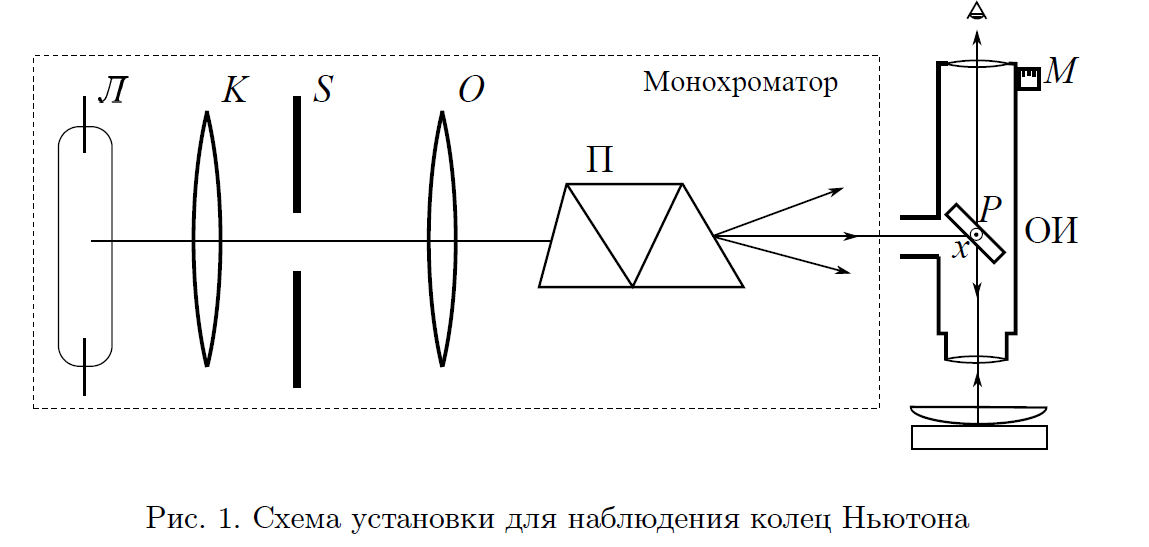
\includegraphics[width = 12 cm]{ust.png}
	
\end{figure}


Источником света служит ртутная лампа, находящаяся в защит-
ном кожухе. Для получения монохроматического света применяется
призменный монохроматор, состоящий из конденсора K, коллимато-
ра (щель S и объектив O) и призмы прямого зрения П. Эти устрой-
ства с помощью рейтеров располагаются на оптической скамье. Свет от
монохроматора попадает на опак-иллюминатор (ОИ), расположенный
между окуляром и объективом микроскопа специальное устройство
для освещения объекта при работе в отражённом свете. Внутри опак-
иллюминатора находится полупрозрачная пластинка P, наклоненная
под углом $45^O$ к оптической оси микроскопа.


\section{Ход работы}

\textbf{Определение радиуса кривизны линзы}
1) Добиваясь наилучшей видимости колец, настроили микроскоп и монохроматор.\\
2) Установив перекрестие на середину крайнего левого кольца, начнем двигаться вправа, записывая координату каждого кольца. \\
3) Проделаем это для светлых и темных колец.\\
4) Также, используя сетку 0.01 мм, найдем цену деления нашей объектной шкалы, совместив ее деления с сеткой: 0.001 мм \\
\begin{tabular}{|c|c|c|c|c|}
\hline 
Темные & N & Left q, дел & Right q, дел & $r_{m} ^2*10, mm^2$ \\ 
\hline 
 & 10 & 54 & 765 & 1.26 \\ 
\hline 
 & 9 & 76 & 750 & 1.13 \\ 
\hline 
 & 8 & 92 & 728 & 1.01 \\ 
\hline 
 & 7 & 114 & 707 & 0.88 \\ 
\hline 
 & 6 & 139 & 677 & 0.72 \\ 
\hline 
 & 5 & 166 & 655 & 0.6 \\ 
\hline 
 & 4 & 195 & 625 & 0.46 \\ 
\hline 
 & 3 & 230 & 588 & 0.32 \\ 
\hline 
 & 2 & 270 & 541 & 0.18 \\ 
\hline 
 & 1 & 318 & 507 & 0.09 \\ 
\hline 
 & 0 & 411 & 411 & • \\ 
\hline 
Светлые & 10 & 97 & 832 & 1.35 \\ 
\hline 
 & 9 & 106 & 814 & 1.25 \\ 
\hline 
 & 8 & 137 & 792 & 1.06 \\ 
\hline 
 & 7 & 157 & 770 & 0.94 \\ 
\hline 
 & 6 & 177 & 749 & 0.82 \\ 
\hline 
 & 5 & 207 & 722 & 0.66 \\ 
\hline 
 & 4 & 234 & 692 & 0.52 \\ 
\hline 
 & 3 & 265 & 658 & 0.38 \\ 
\hline 
 & 2 & 304 & 622 & 0.25 \\ 
\hline 
 & 1 & 354 & 571 & 0.12 \\ 
\hline 
 & 0 & 468 & 468 & • \\ 
\hline 
\end{tabular} 
        
        
 \newpage
Построим по ней график: \\
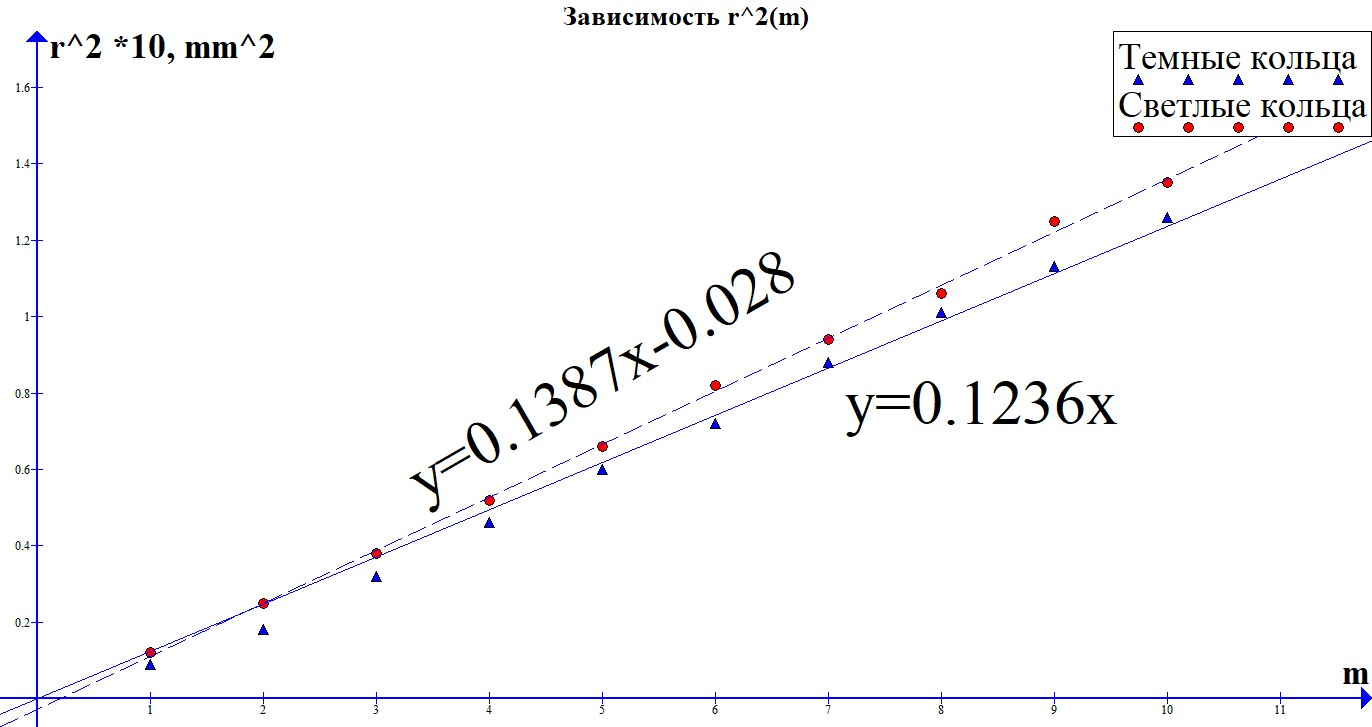
\includegraphics[scale=0.33]{4211}

5) Зная формулы темных и светлых максимумов: $r_{mt}=\sqrt{\lambda_{zel} R m}    $       $   r_{ms}=\sqrt{R \lambda_{\text{желт}}(m-0.5)} $, определим радиус кривизны линзы:\\
$R_1$ = 2.33 cm\\
$R_2$ = 2.39 cm\\
$R=\frac{R_1+R_2}{2} = 2.36 cm $\\
6) Пронаблюдаем биения. Посчитаем количество светлых максимумом до размытой картины. Используя формулу $\bigtriangleup m =\frac{\lambda_2}{2(\lambda_2-\lambda_1}$, найдем длину "темной" волны: $\lambda_1=537 nm$ (длина зеленой волны - $\lambda_{\text{зел}}$=546 nm



































\end{document} % конец документа
